\chapter{Gallery}
\label{cp:Gallery}
\begin{figure}[!htpb]
    \centering
    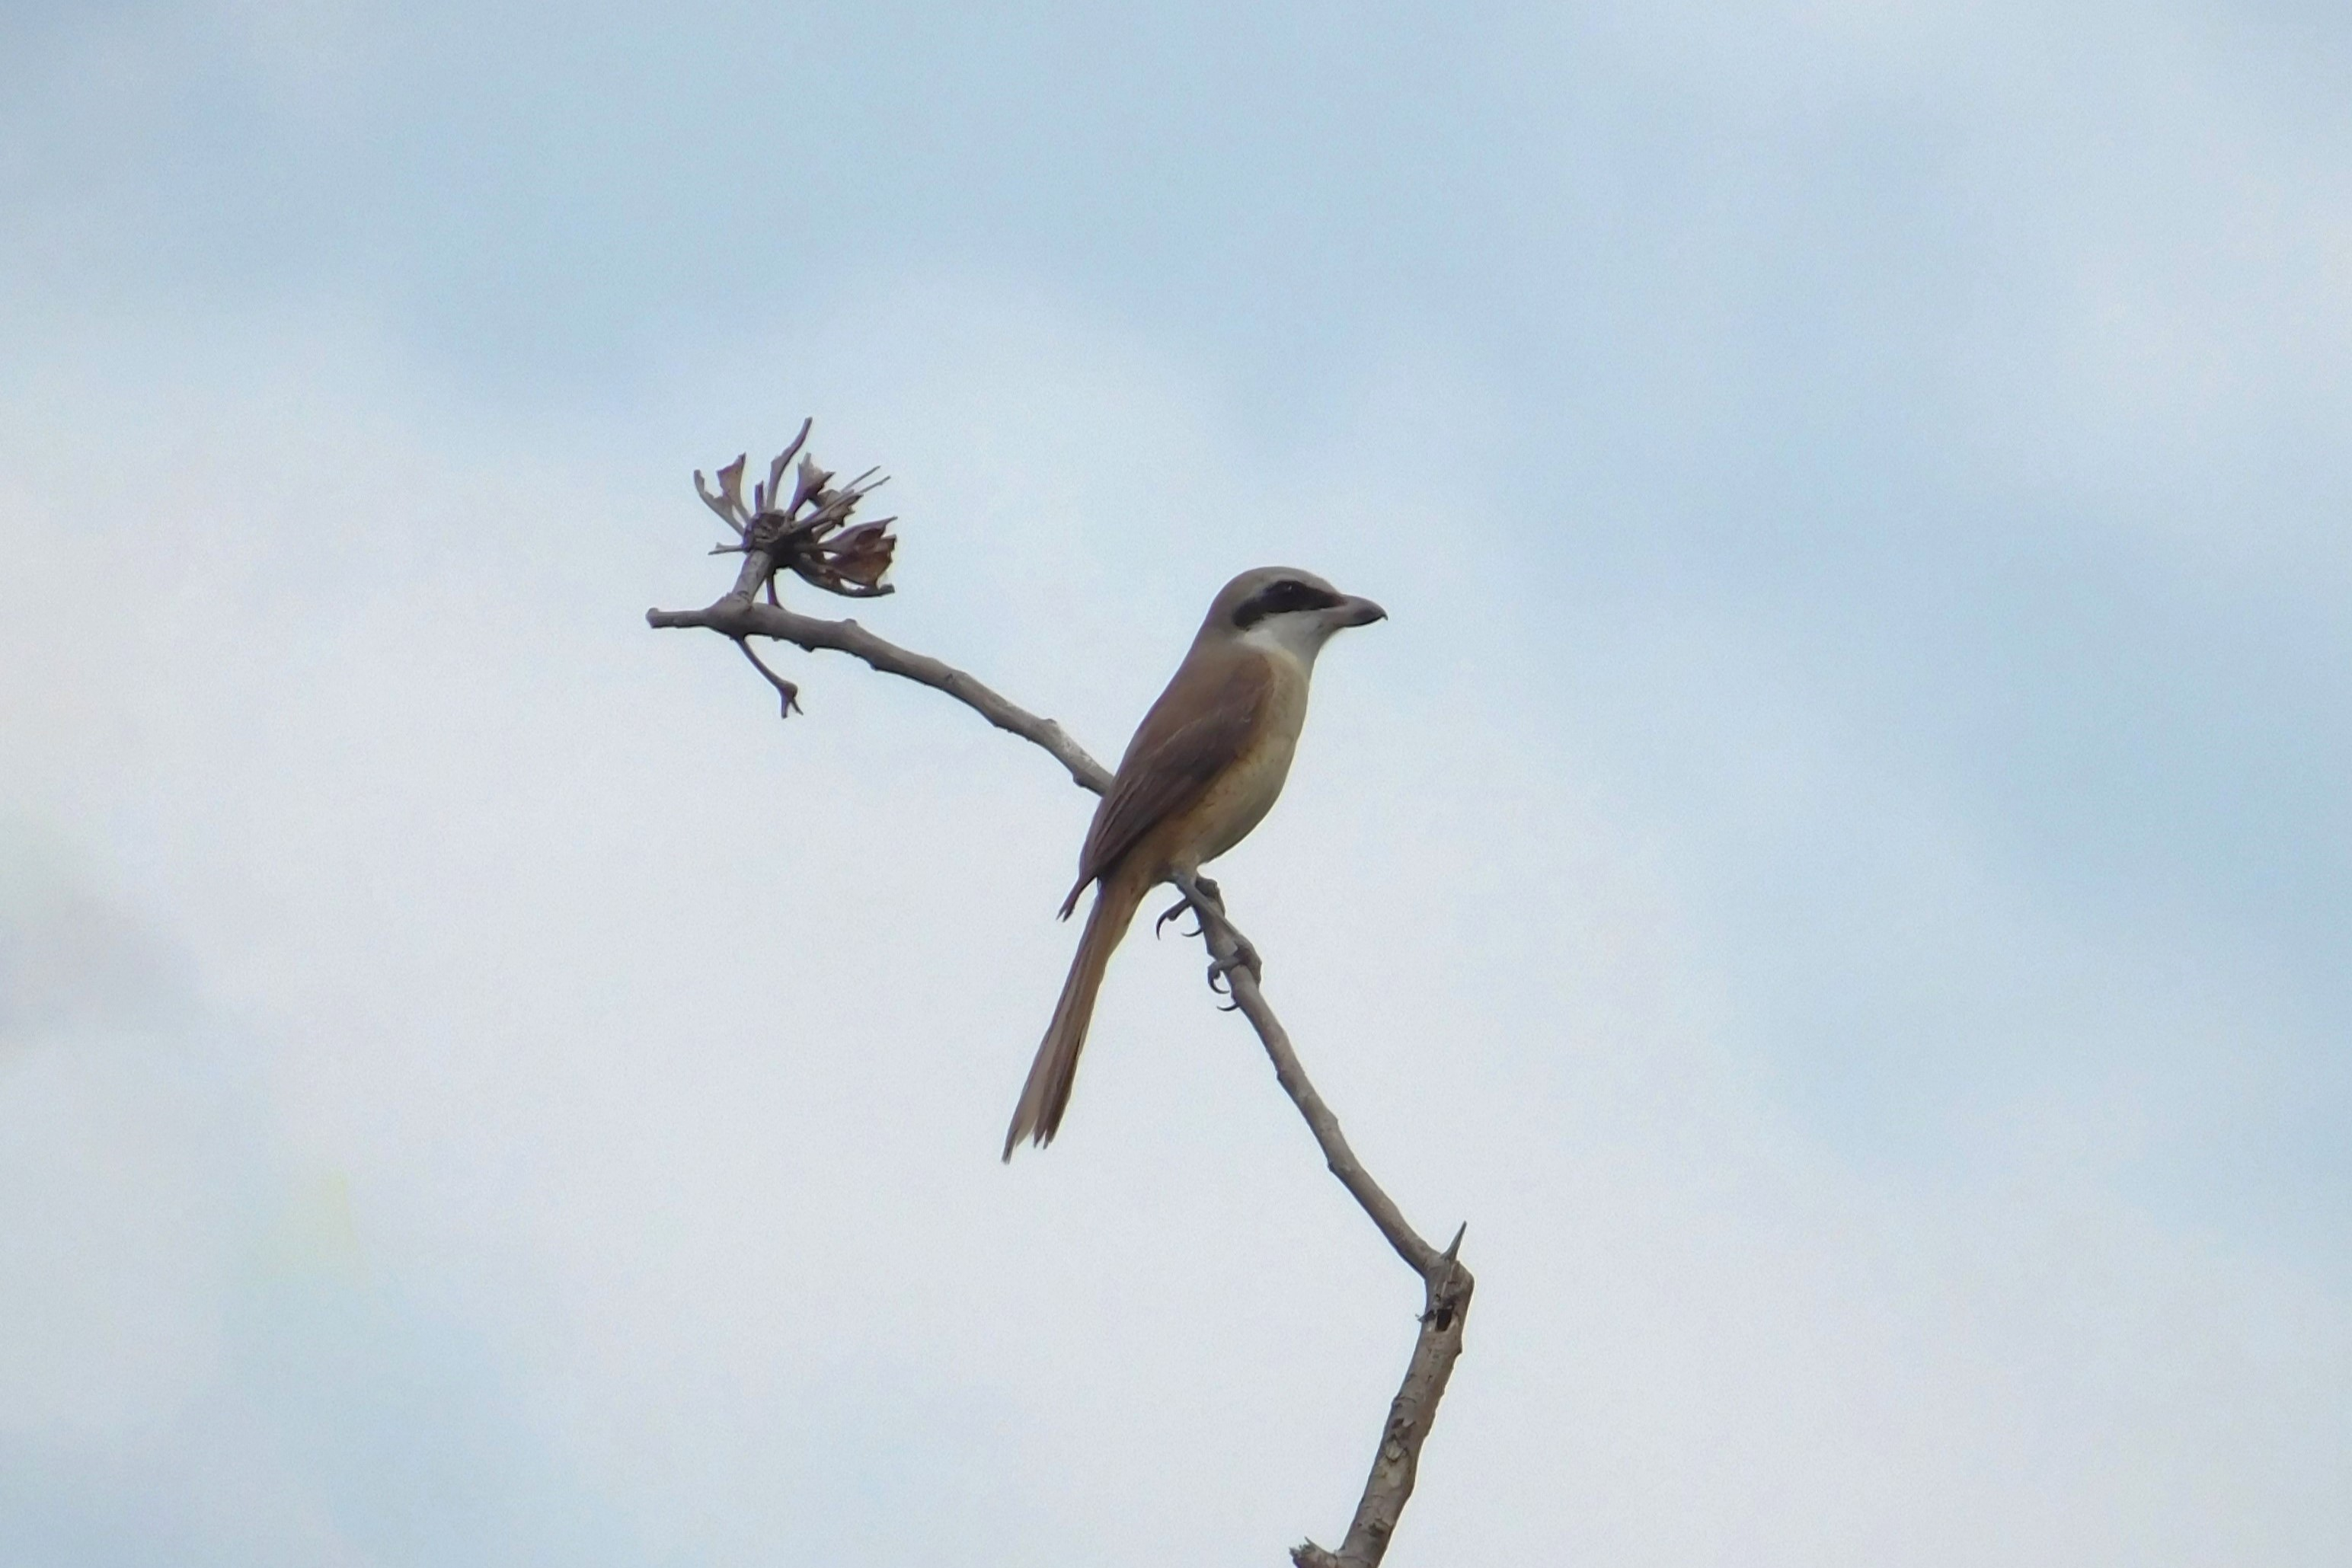
\includegraphics[width=\linewidth]{Figures/brown-shrike.JPG}
    \caption[]{Brown Shrike. Four different sightings throughout the period of study, but only from the exact same location, hotspot 2.}
    \label{fig:figure-01}
\end{figure}
\begin{figure}[!htpb]
    \centering
    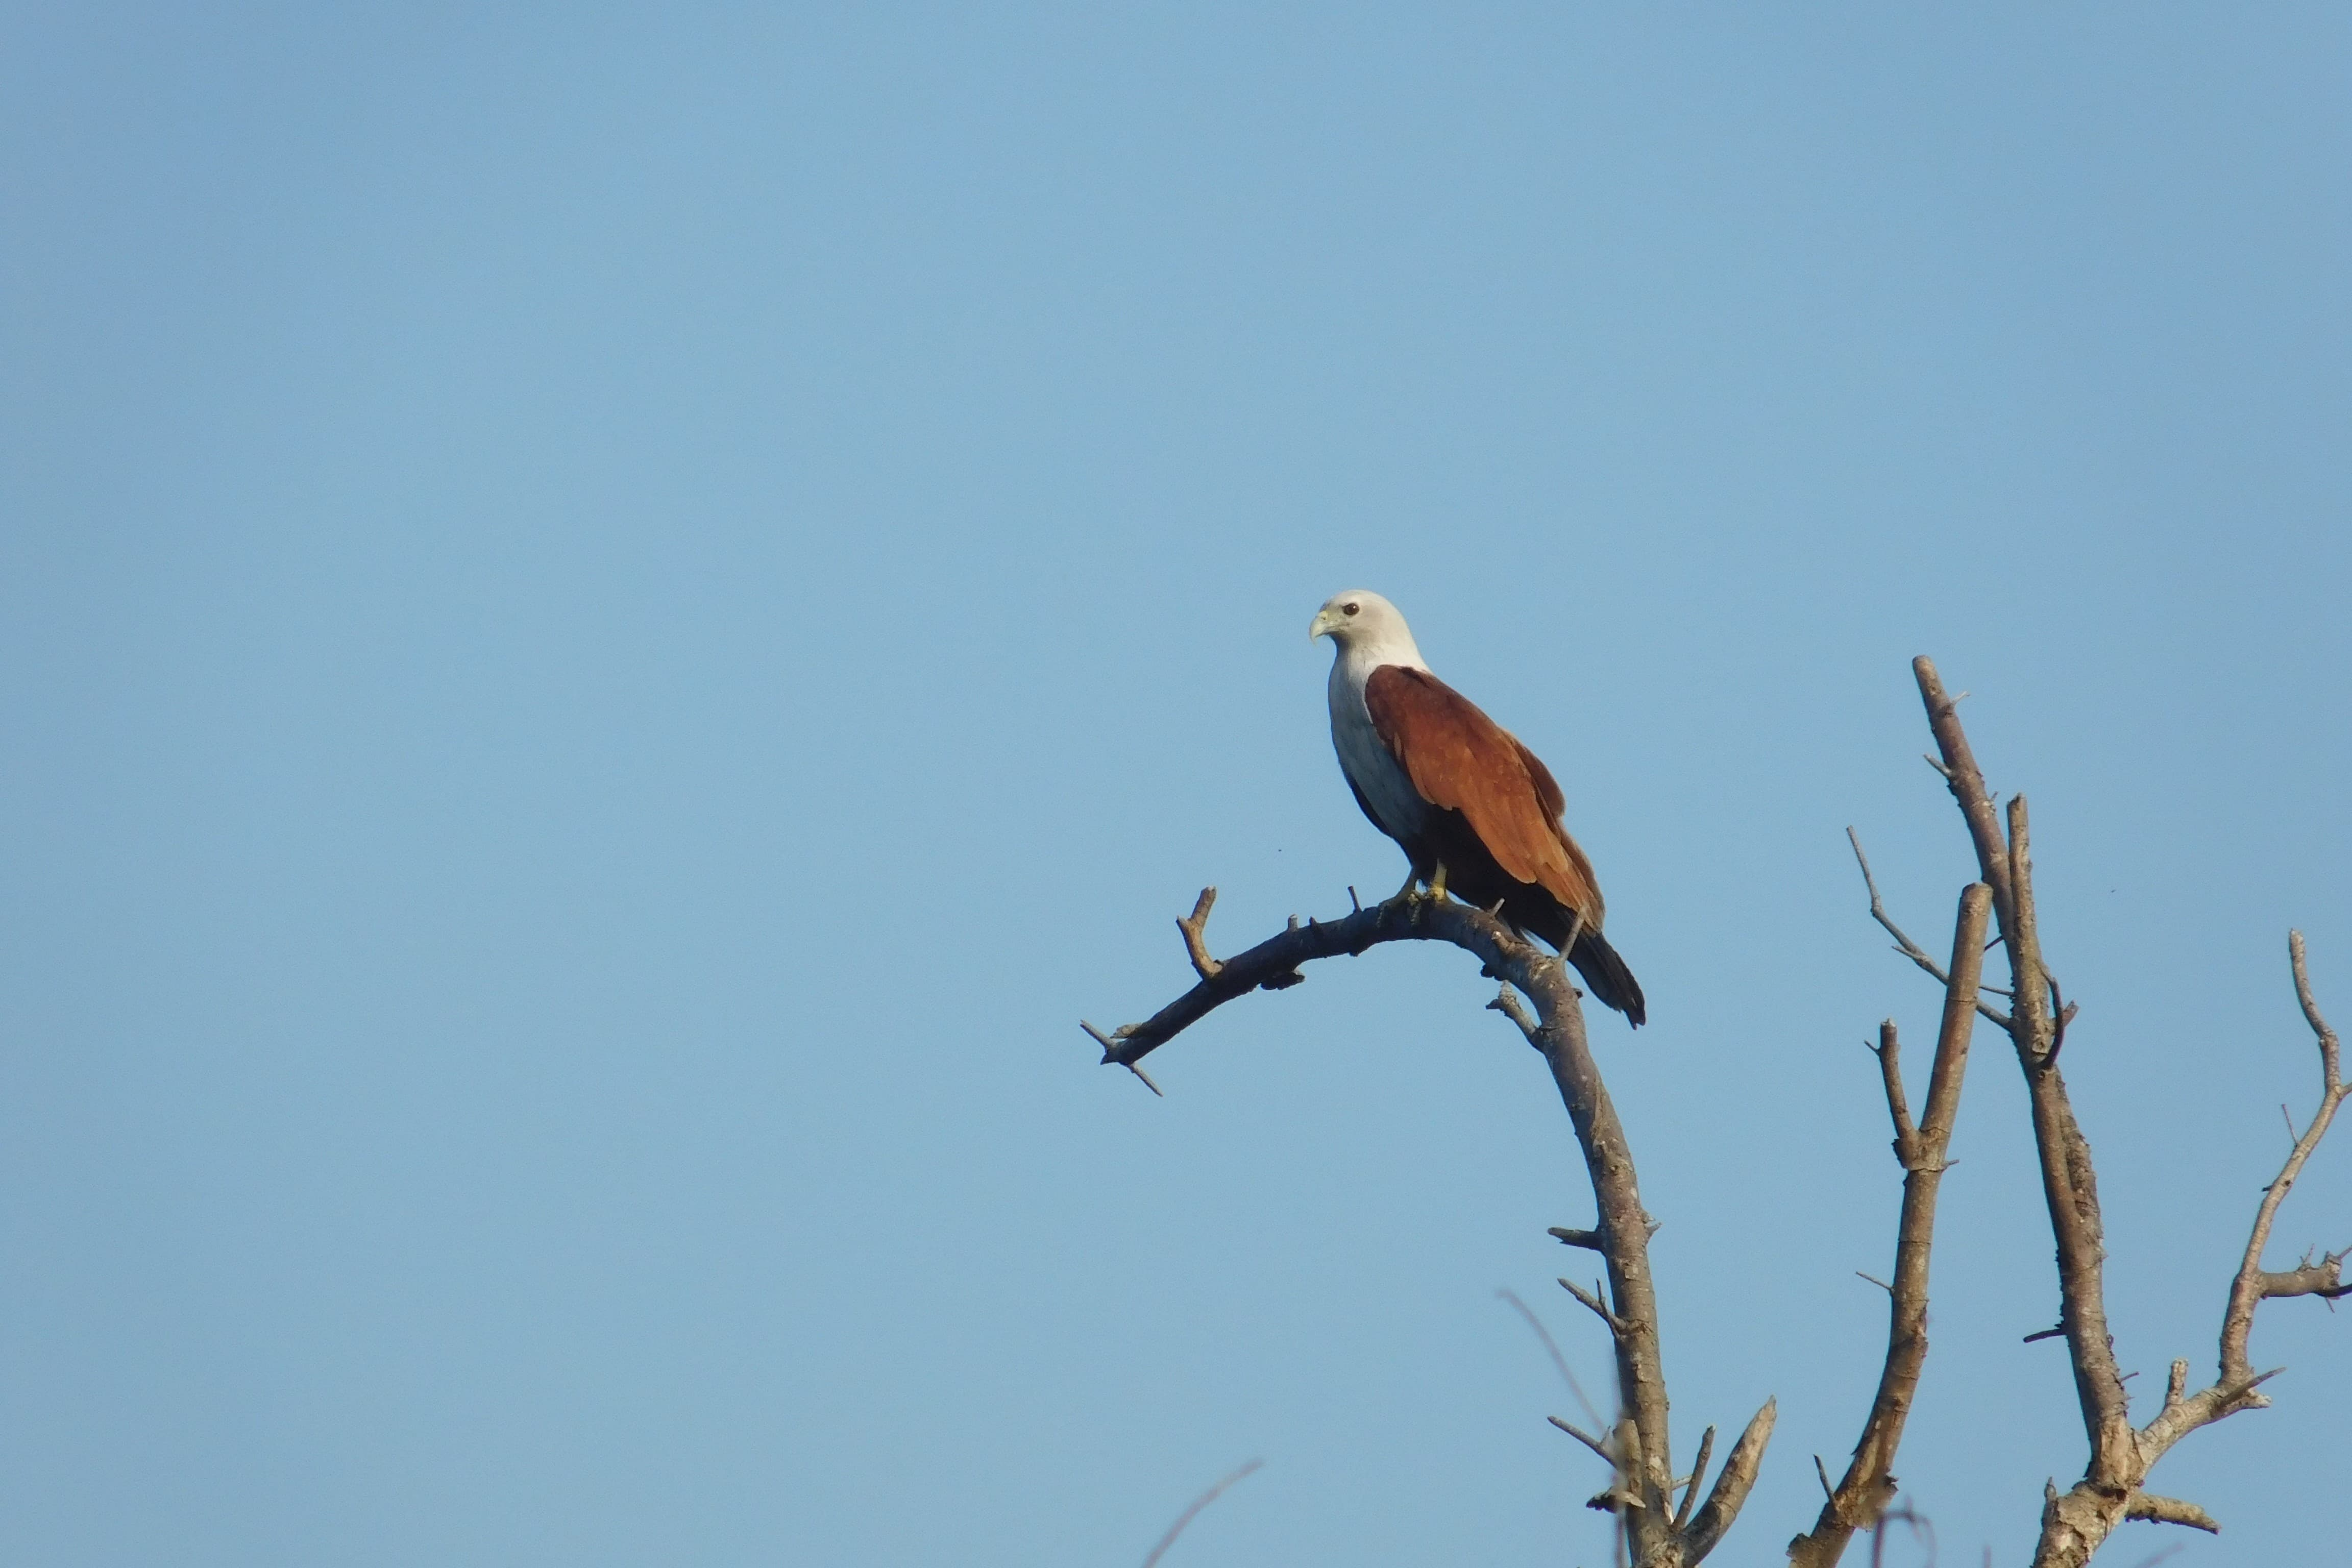
\includegraphics[width=\linewidth]{Figures/brahmini-kite.JPG}
    \caption[]{Brahminy Kite, Kaju kele(hotspot 2).}
    \label{fig:figure-01}
\end{figure}
\begin{figure}[!htpb]
    \centering
    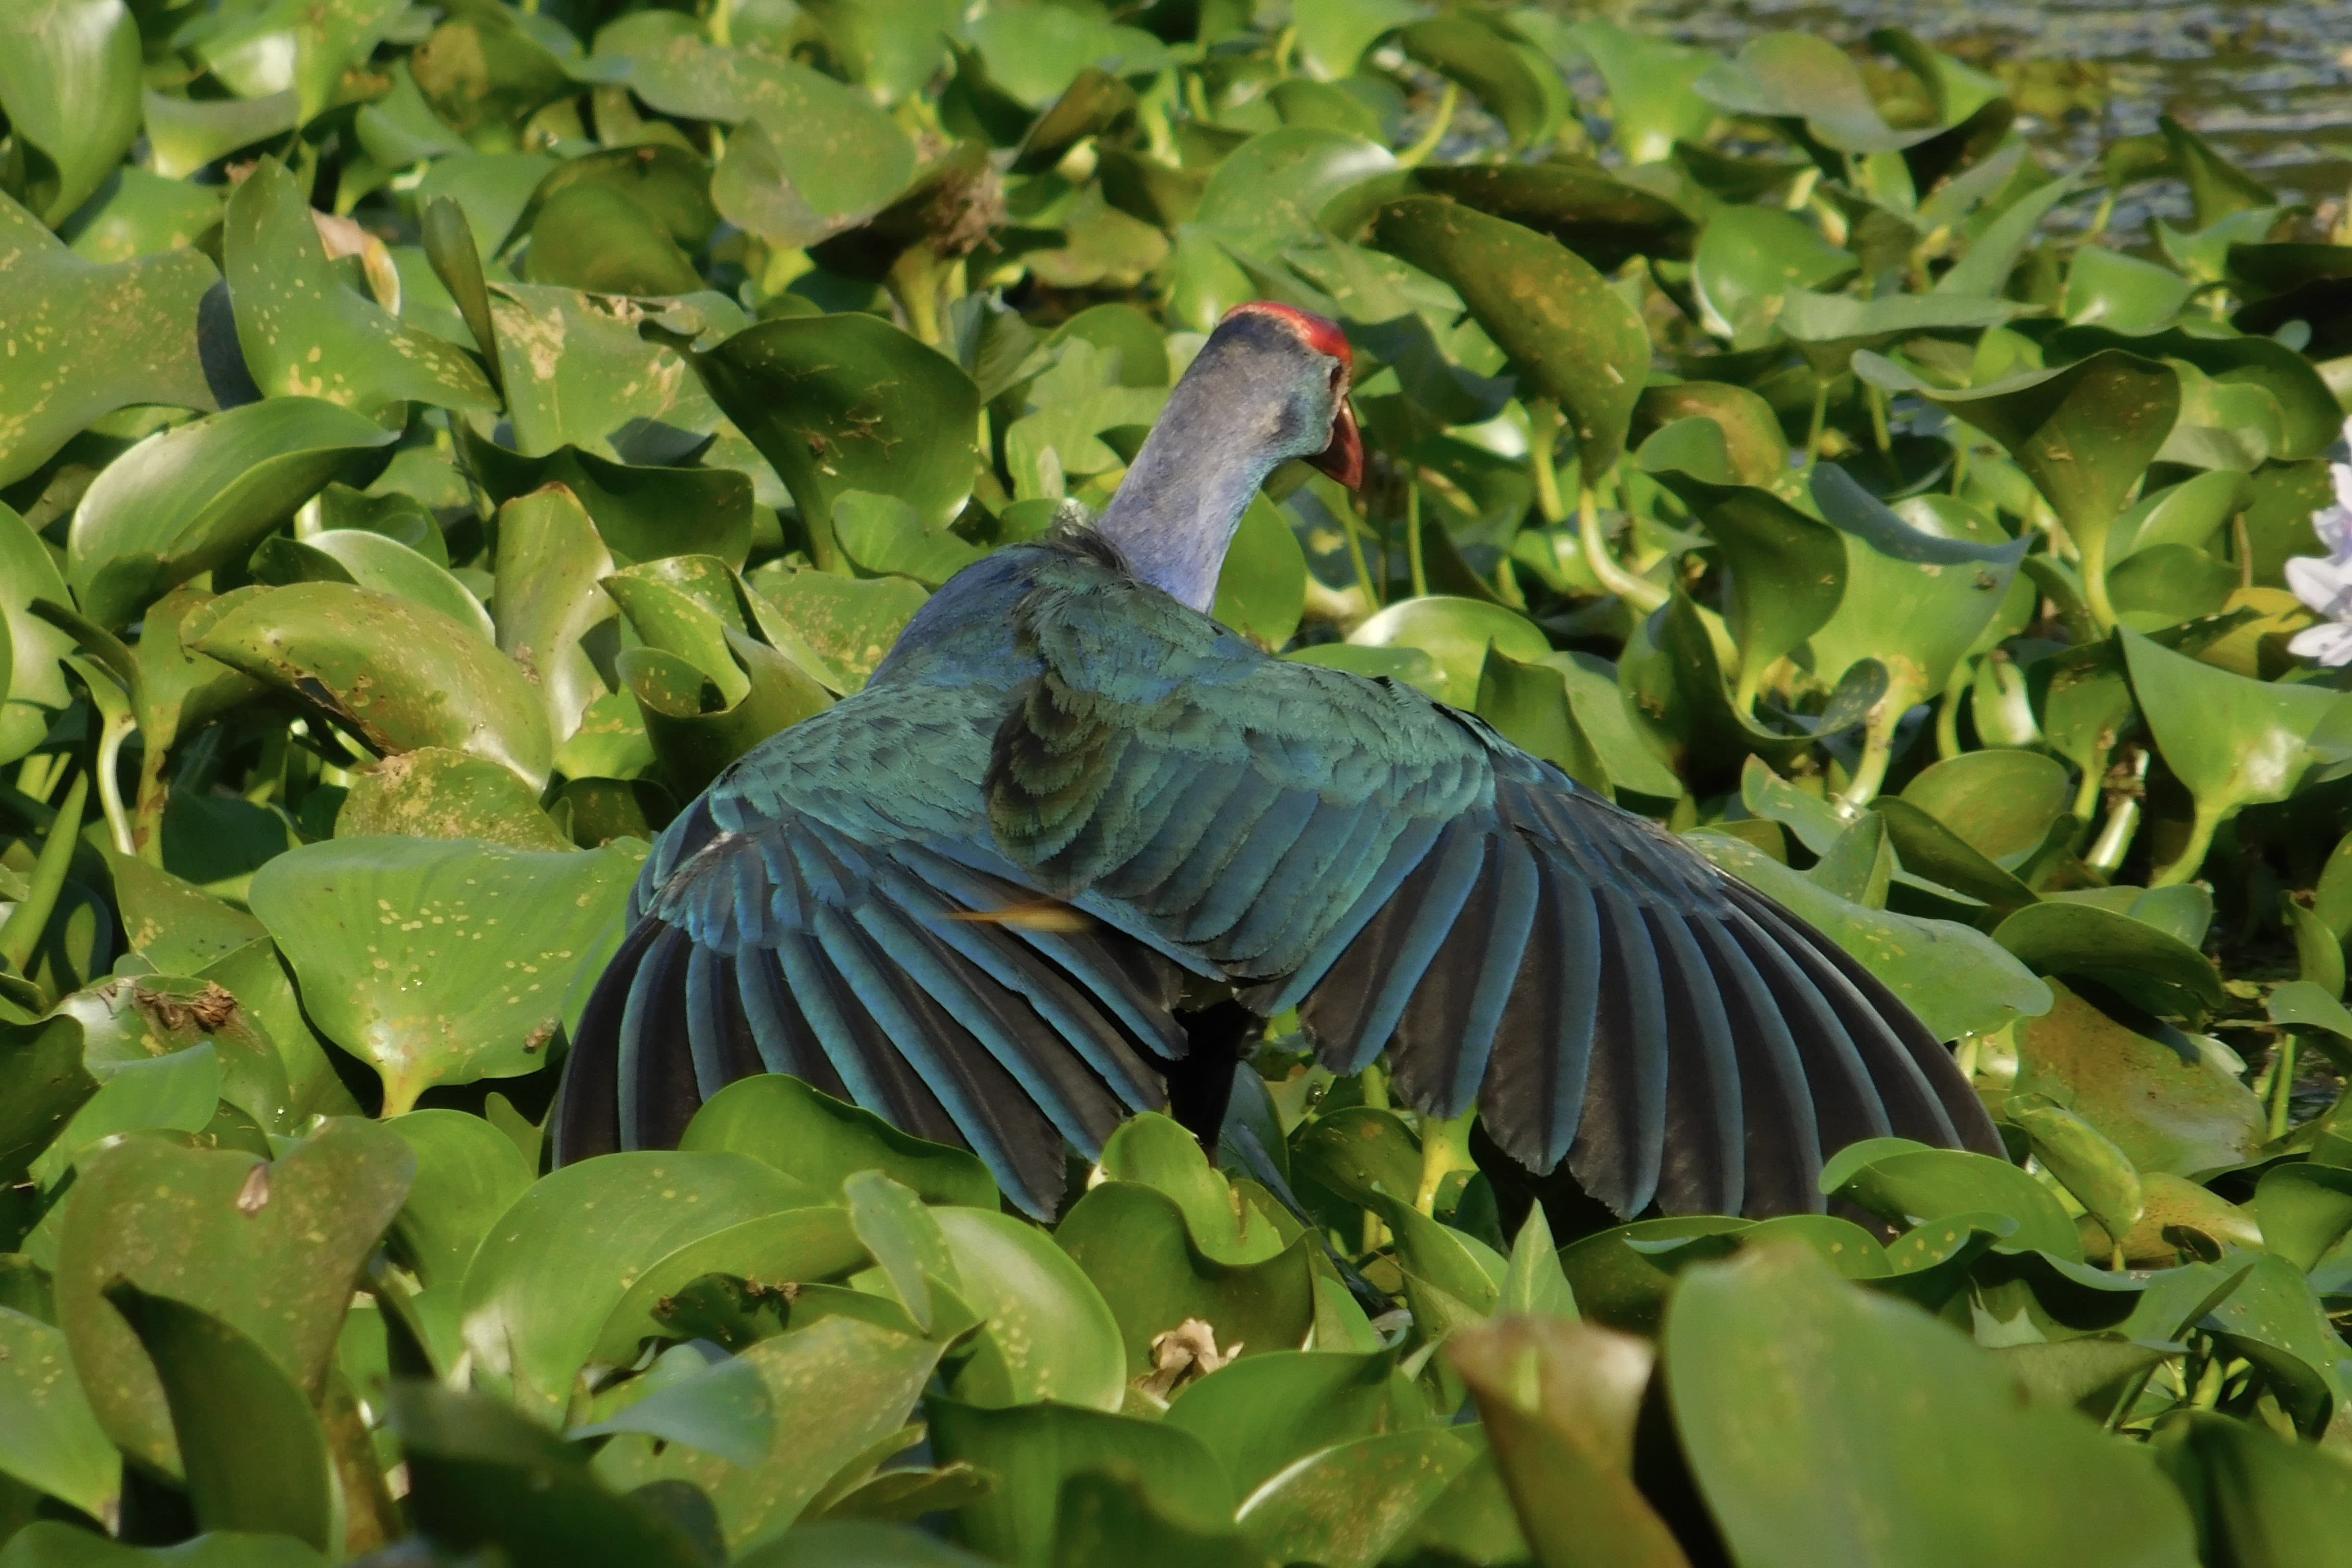
\includegraphics[width=\linewidth]{Figures/swamp-hen.JPG}
    \caption[]{Grey-headed Swamphen drying its feathers, Boat yard.}
    \label{fig:figure-01}
\end{figure}
\begin{figure}[!htpb]
    \centering
    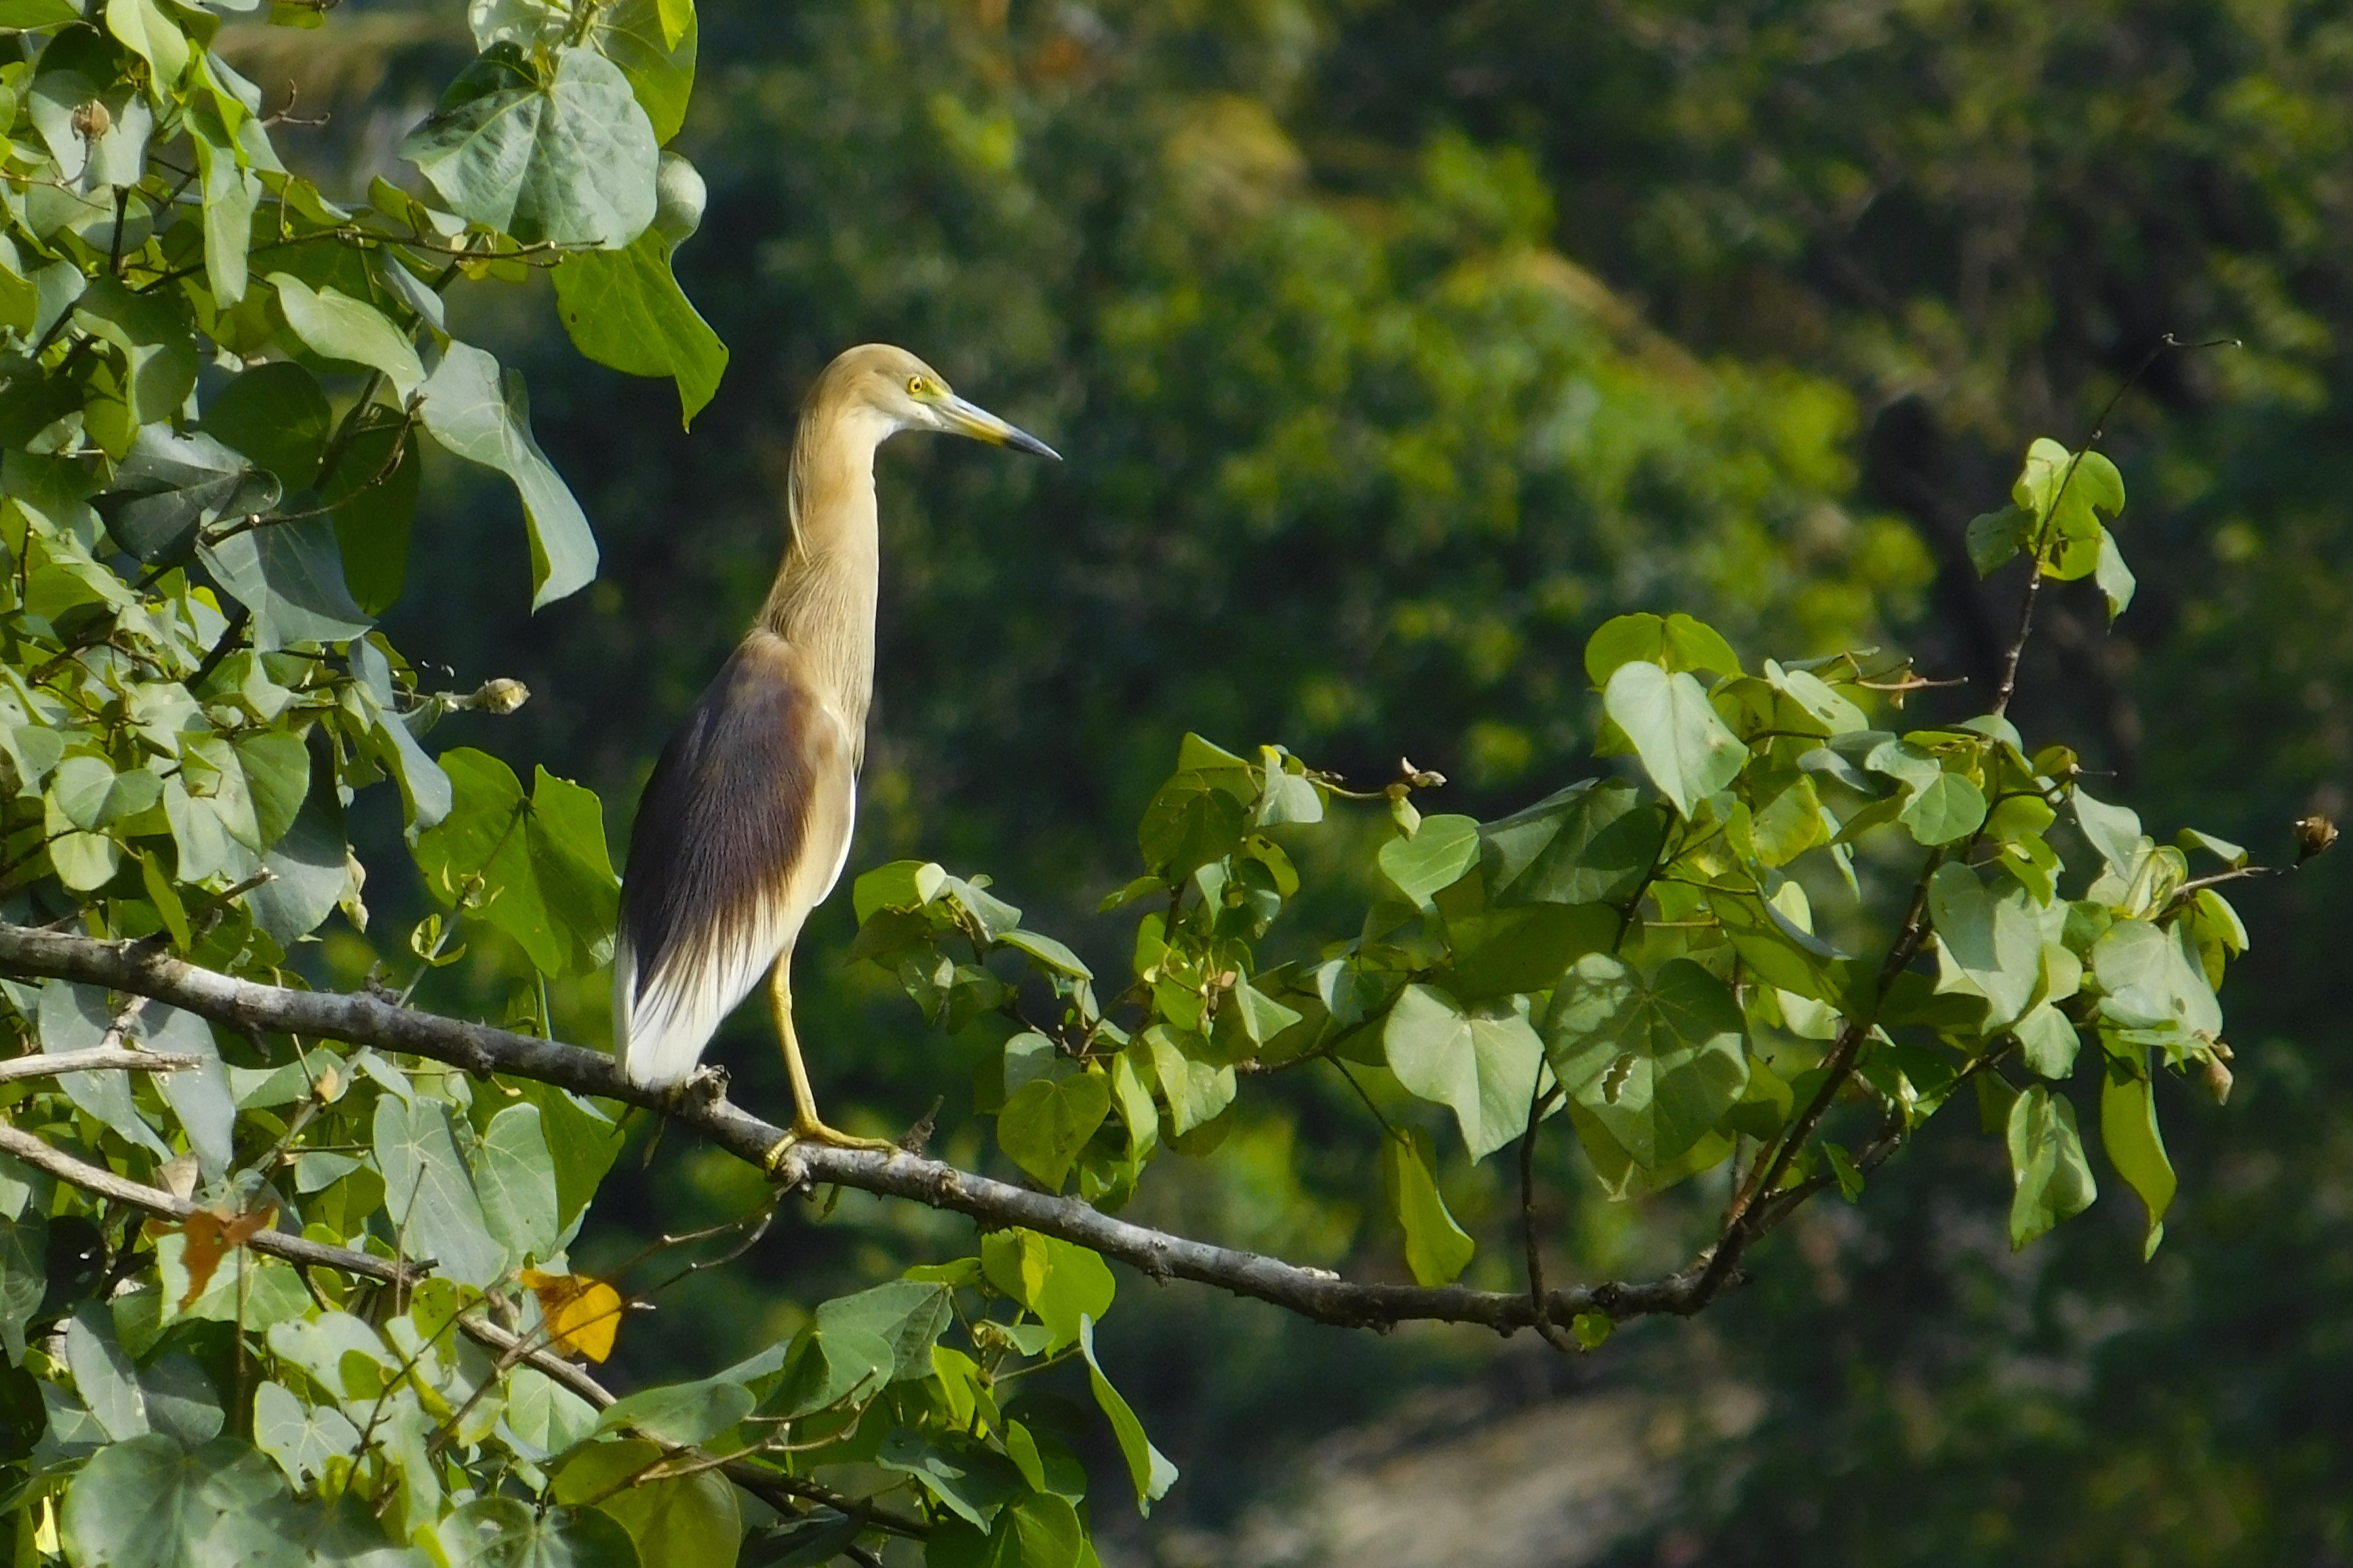
\includegraphics[width=\linewidth]{Figures/pond-heron.JPG}
    \caption[]{An Indian Pond-Heron, boat yard. }
    \label{fig:figure-01}
\end{figure}
\begin{figure}[!htpb]
    \centering
    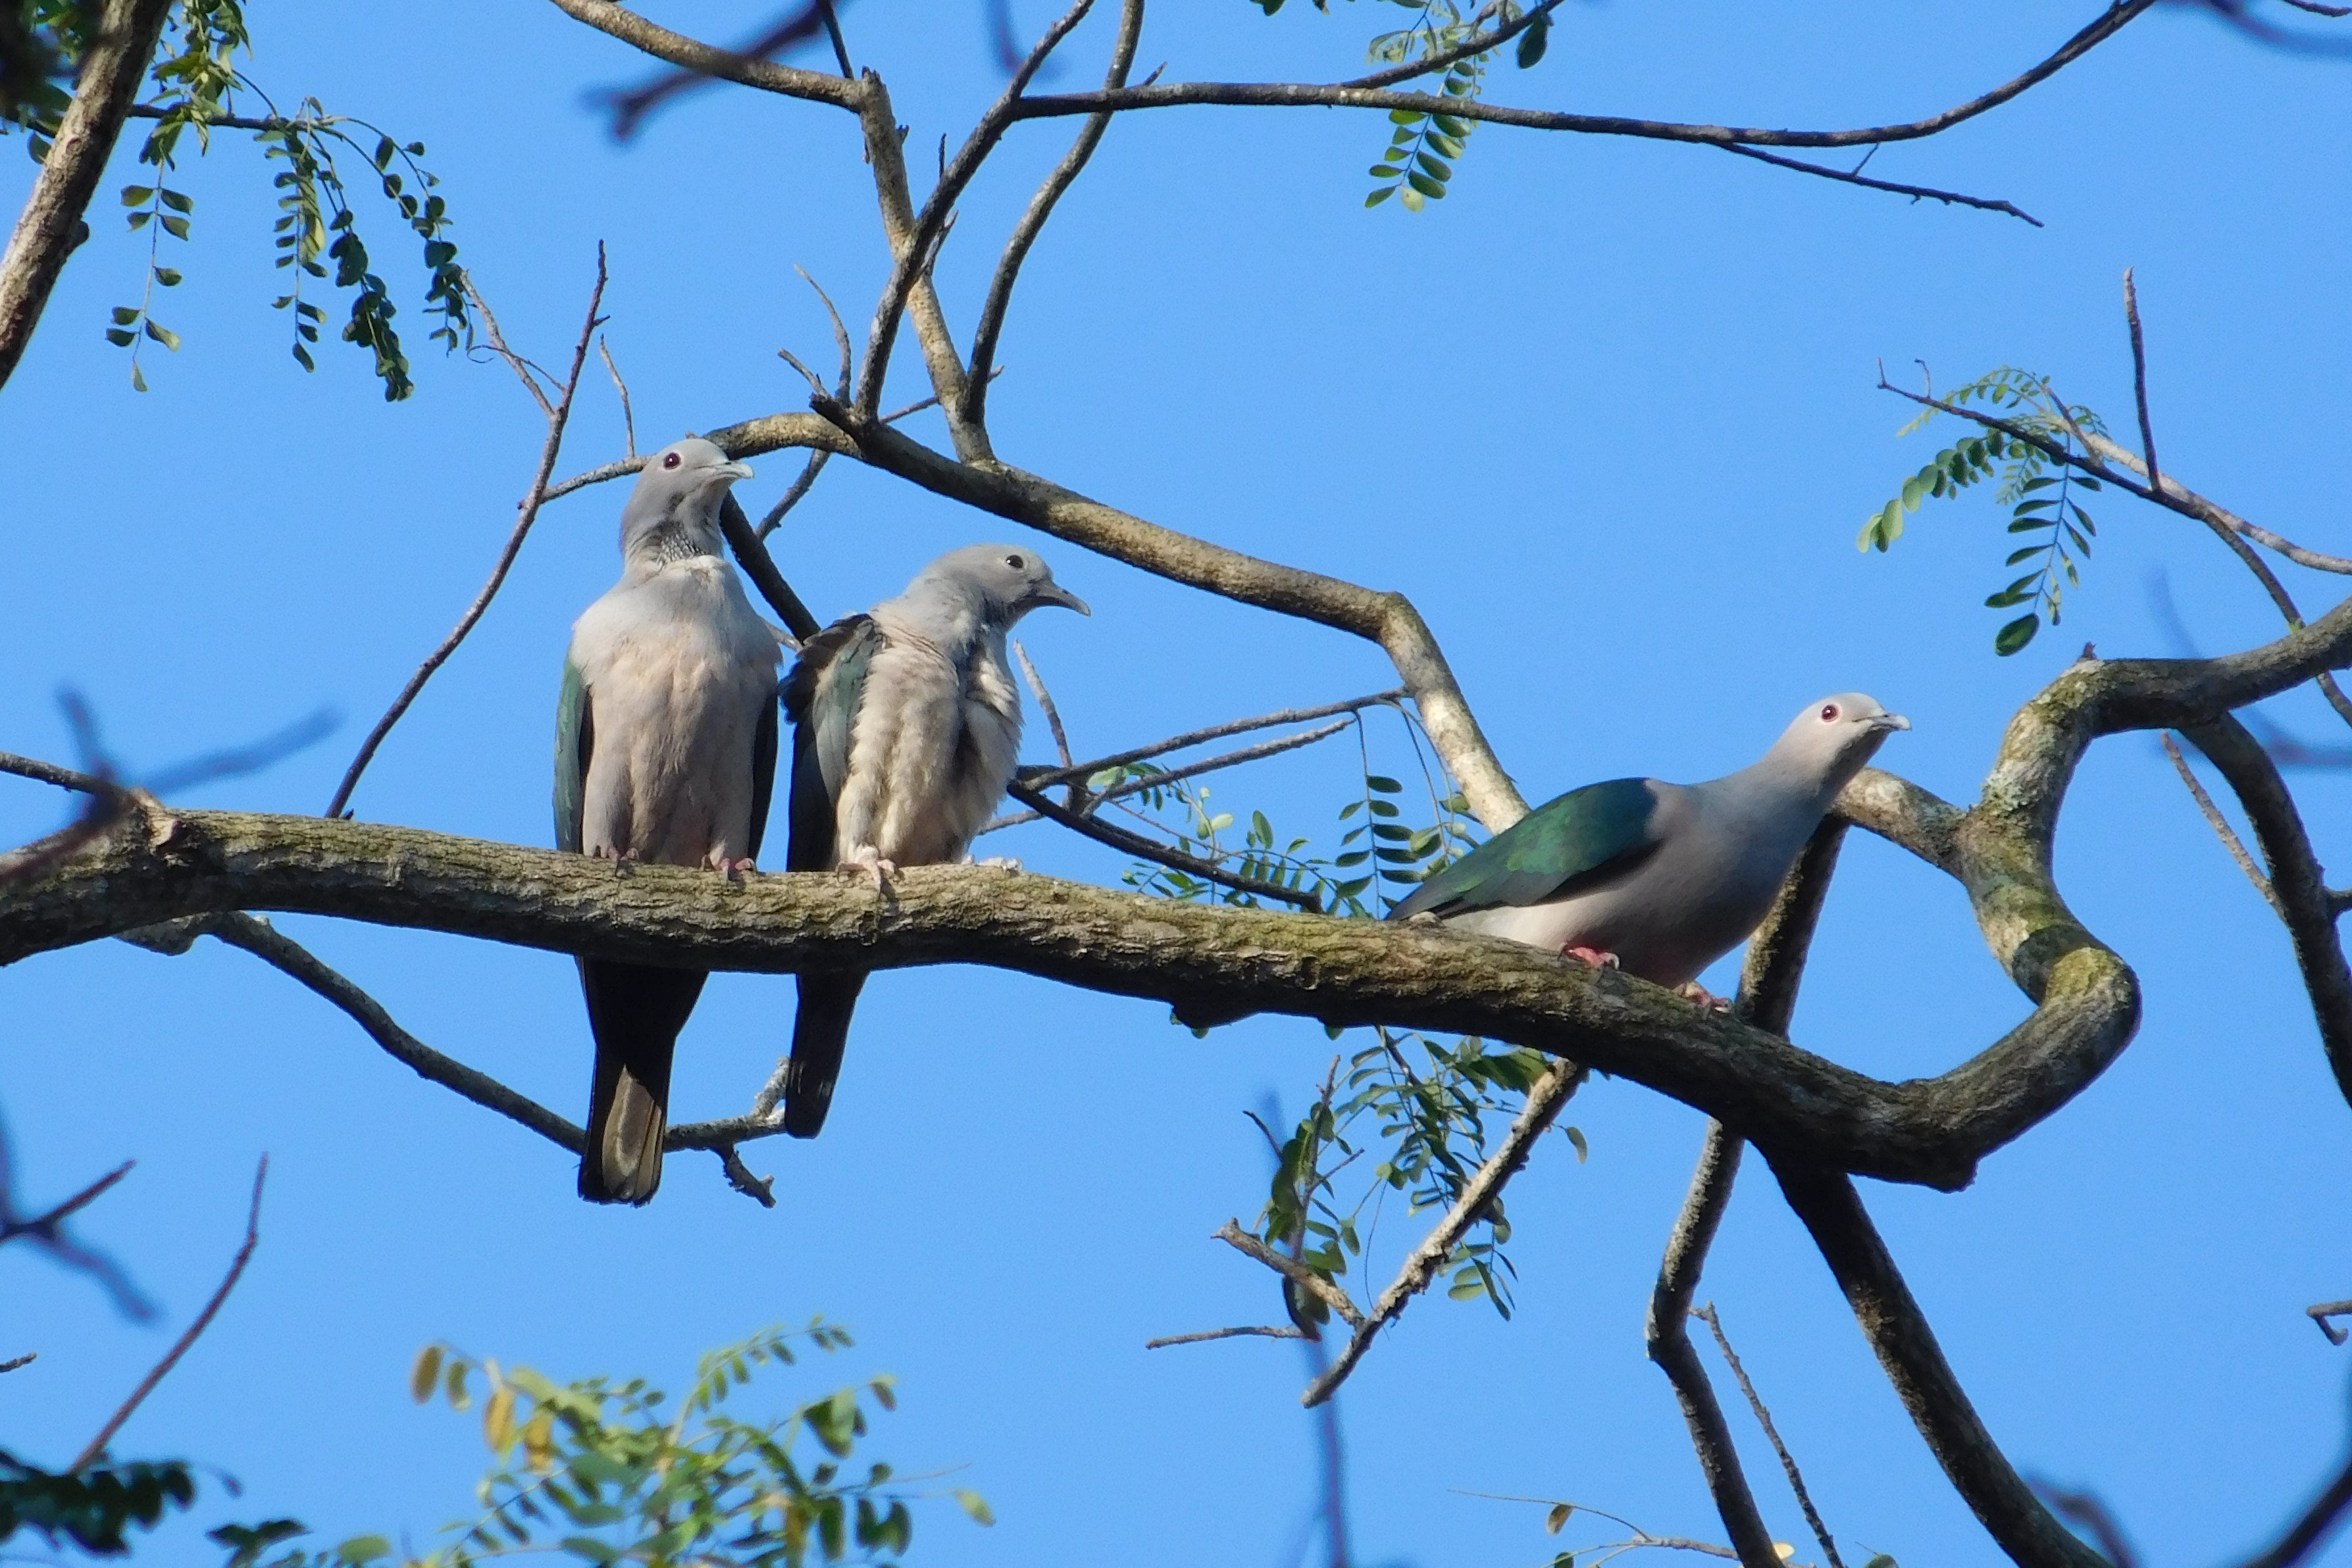
\includegraphics[width=\linewidth]{Figures/imperial-pigeon.JPG}
    \caption[]{Green Imperial-Pigeons, Kaju kele near Dept. of Civil Engineering(hotspot 1).}
    \label{fig:figure-01}
\end{figure}
\begin{figure}[!htpb]
    \centering
    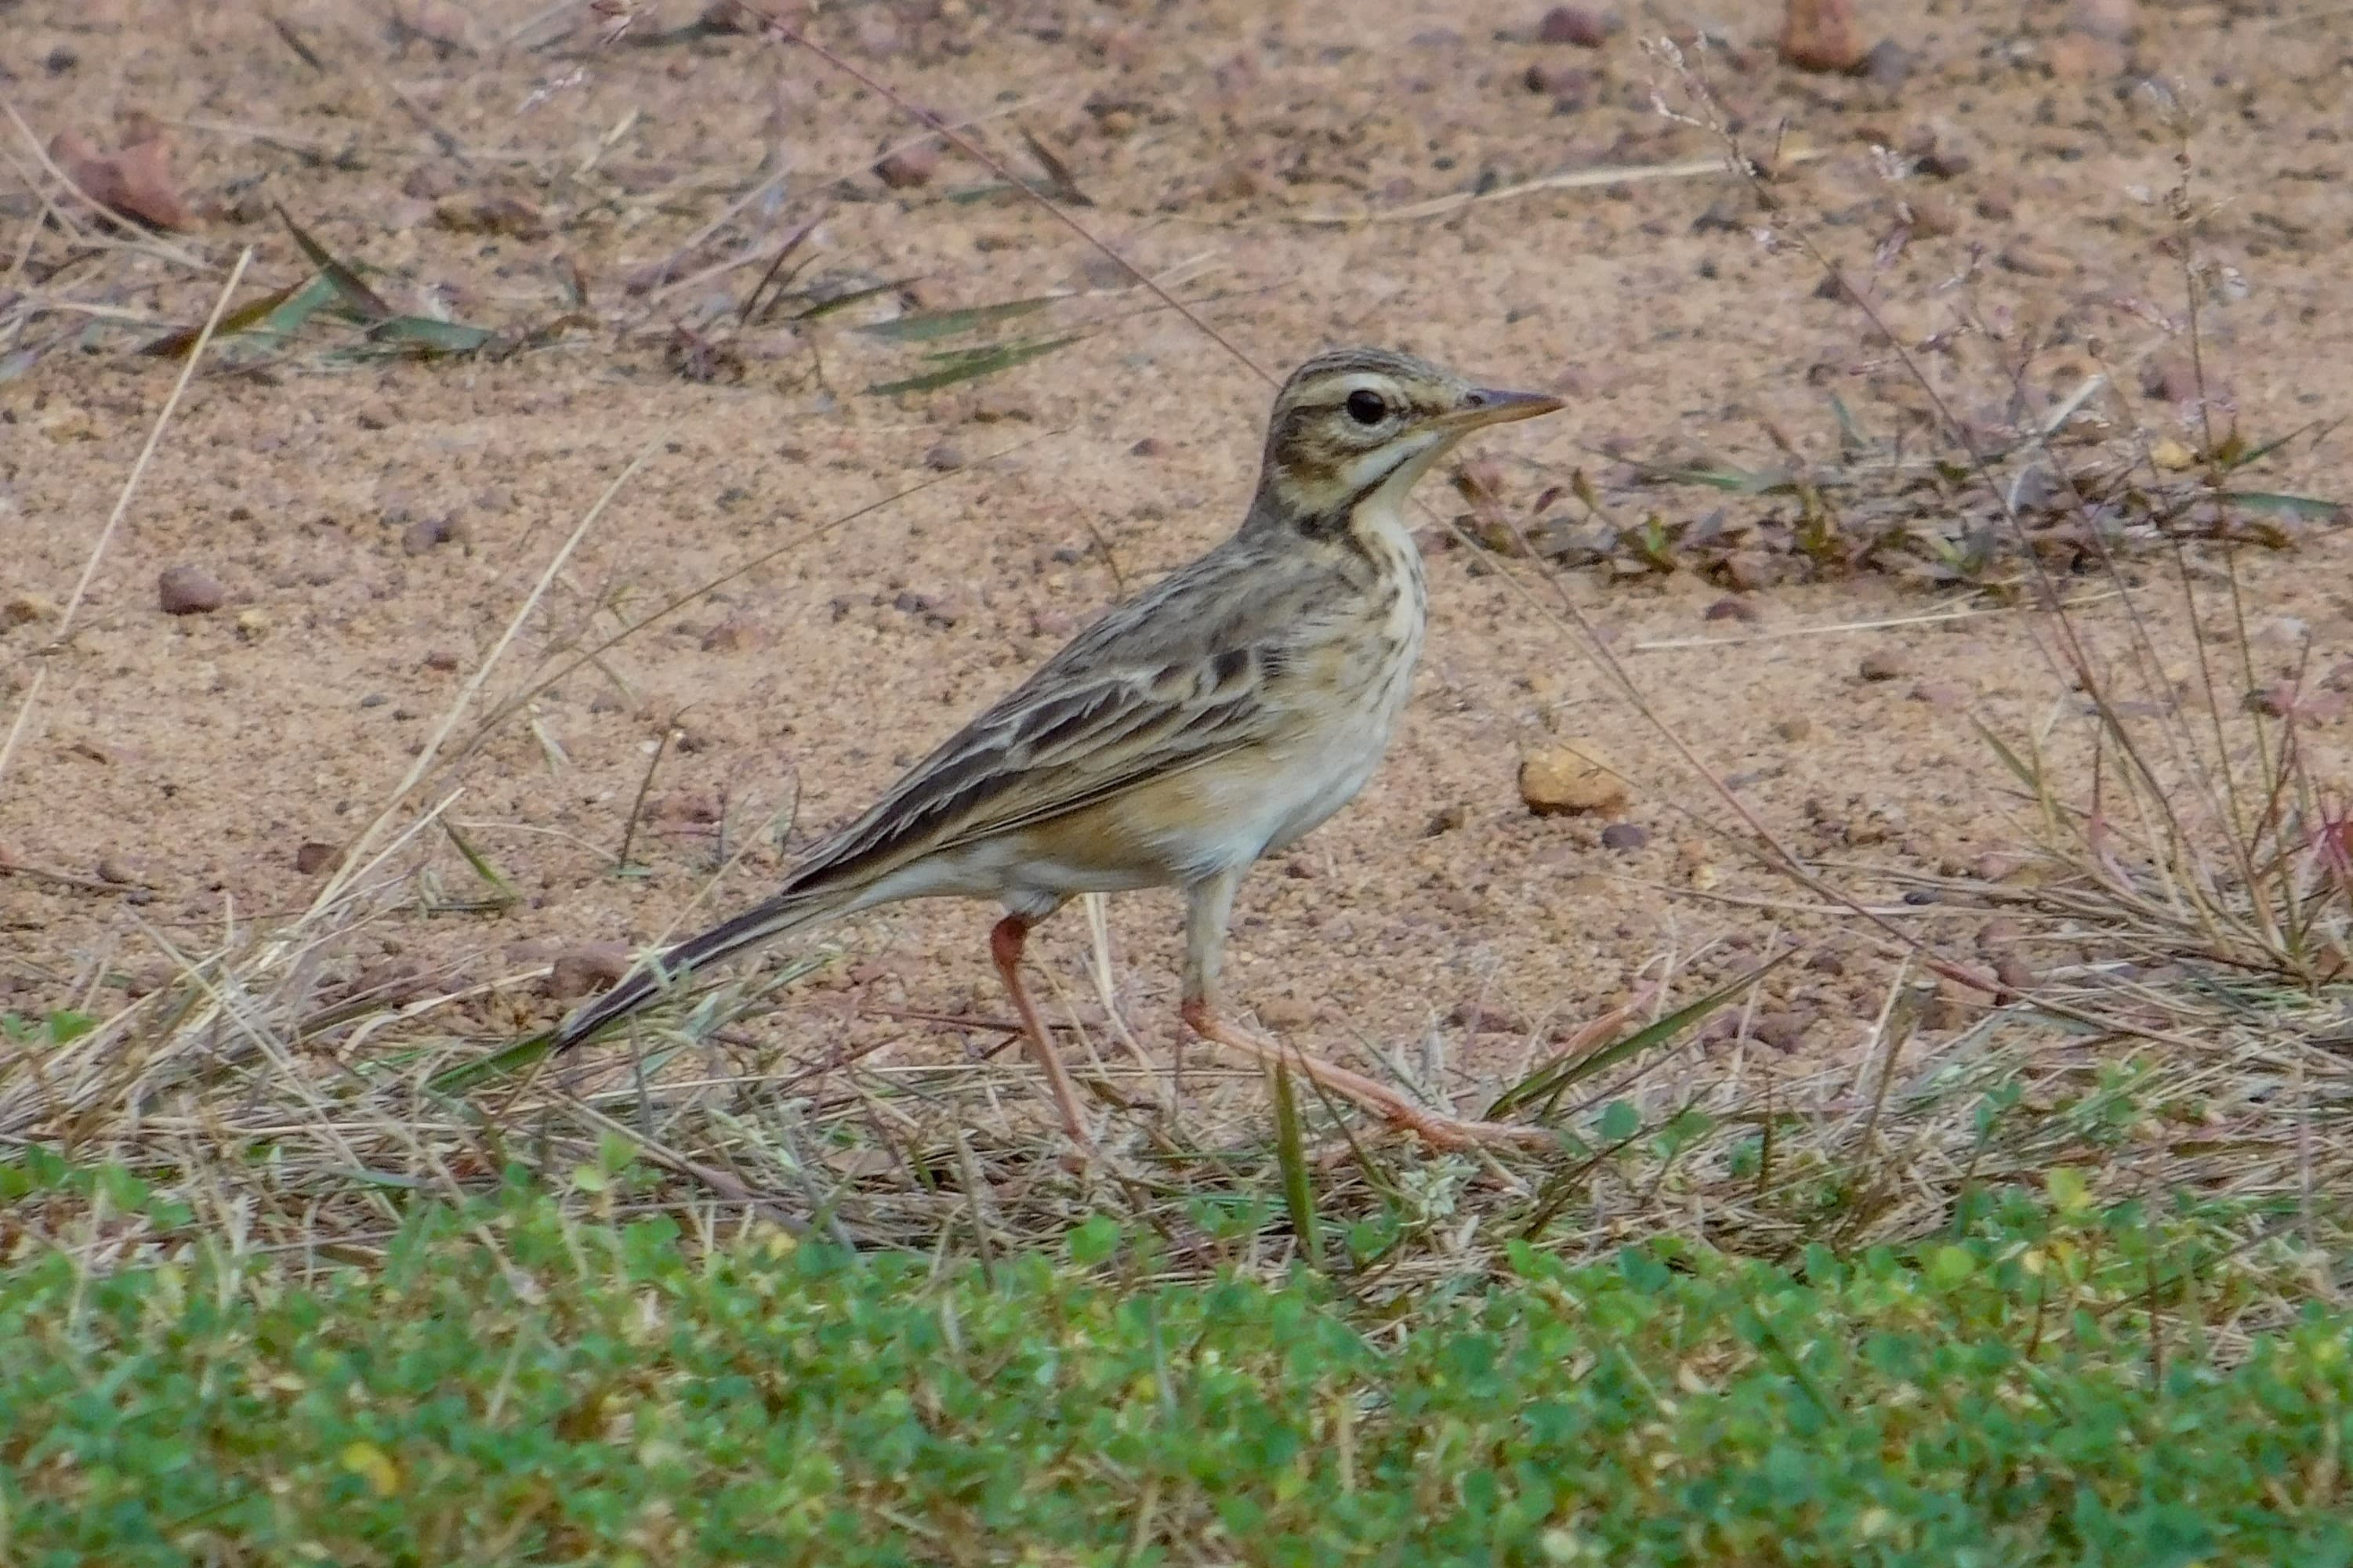
\includegraphics[width=\linewidth]{Figures/pipit.JPG}
    \caption[]{Paddyfield Pipit. University playground.}
    \label{fig:figure-01}
\end{figure}
\begin{figure}[!htpb]
    \centering
    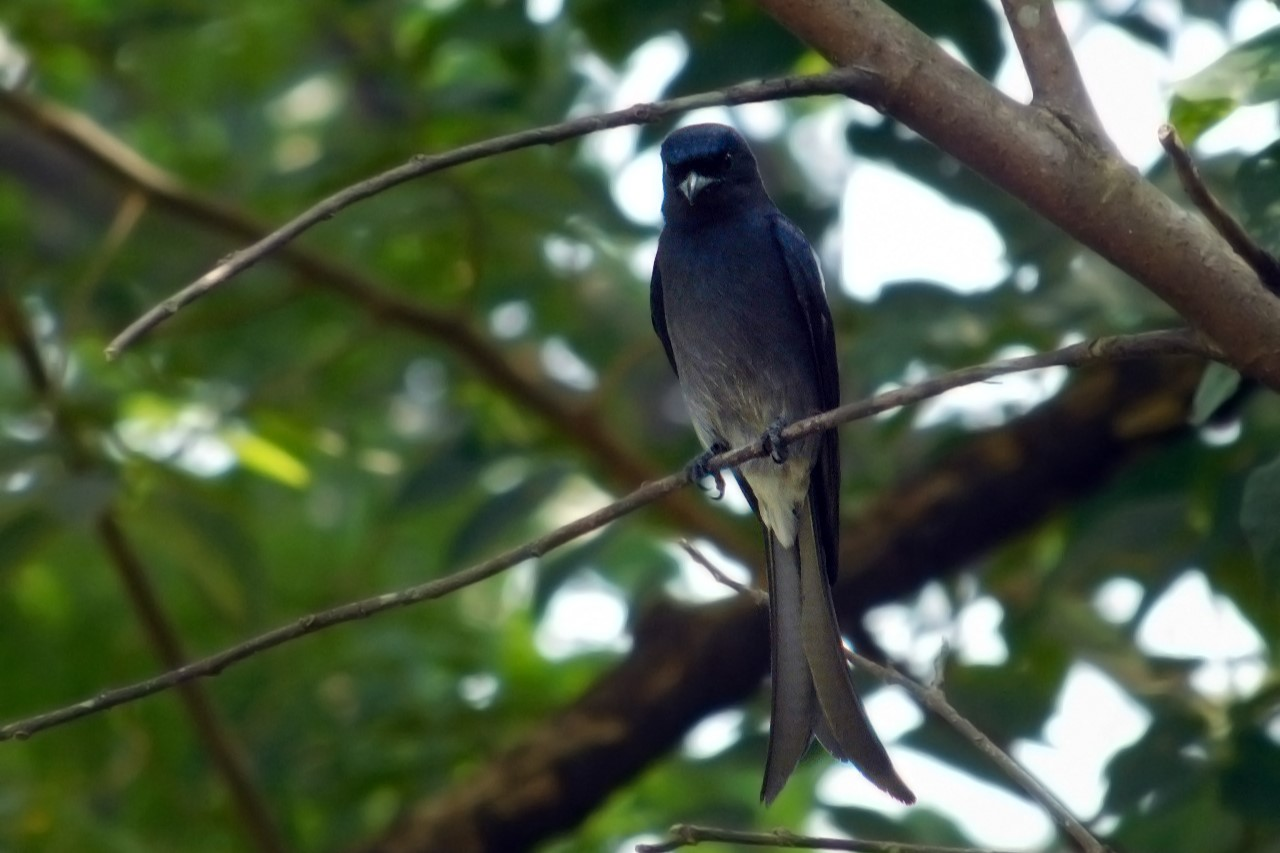
\includegraphics[width=\linewidth]{Figures/drongo.jpg}
    \caption[]{White-bellied Drongo. Kaju kele(hotspot 2).}
    \label{fig:figure-01}
\end{figure}
\begin{figure}[!htpb]
    \centering
    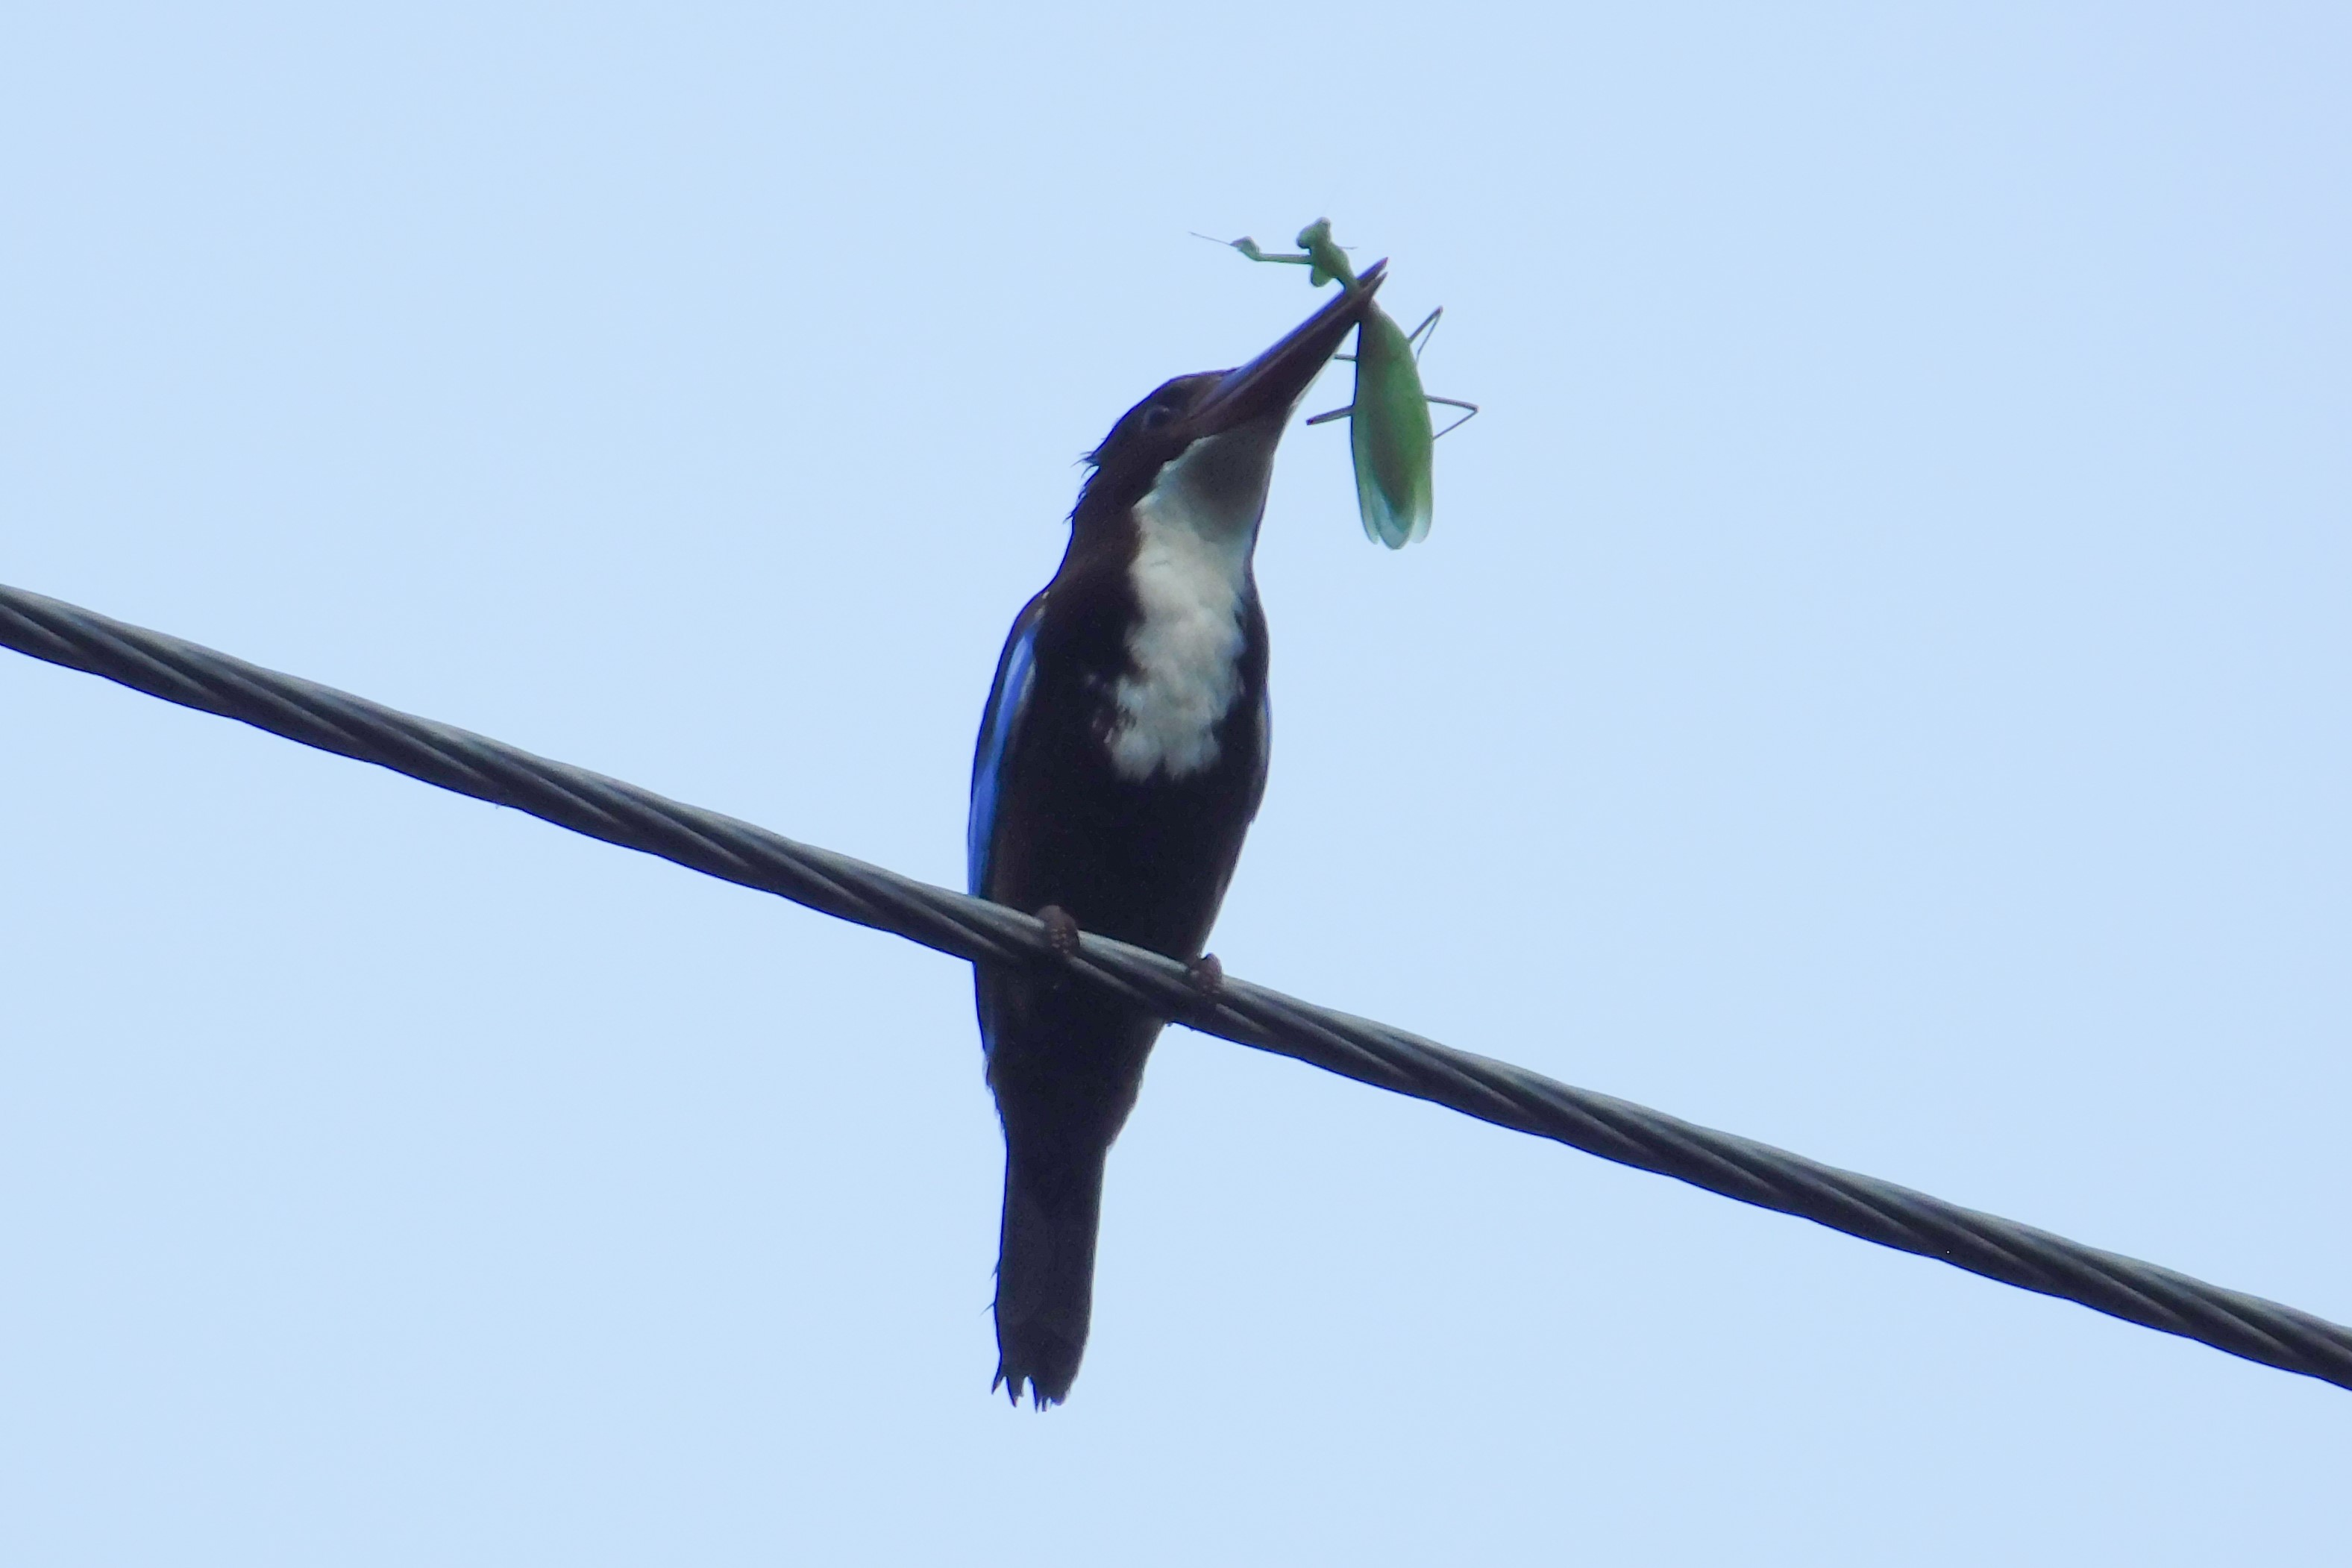
\includegraphics[width=\linewidth]{Figures/kingfisher.JPG}
    \caption[]{A White-breasted Kingfisher preying on a praying mantis, Kaju kele.}
    \label{fig:figure-01}
\end{figure}
\begin{figure}[!htpb]
    \centering
    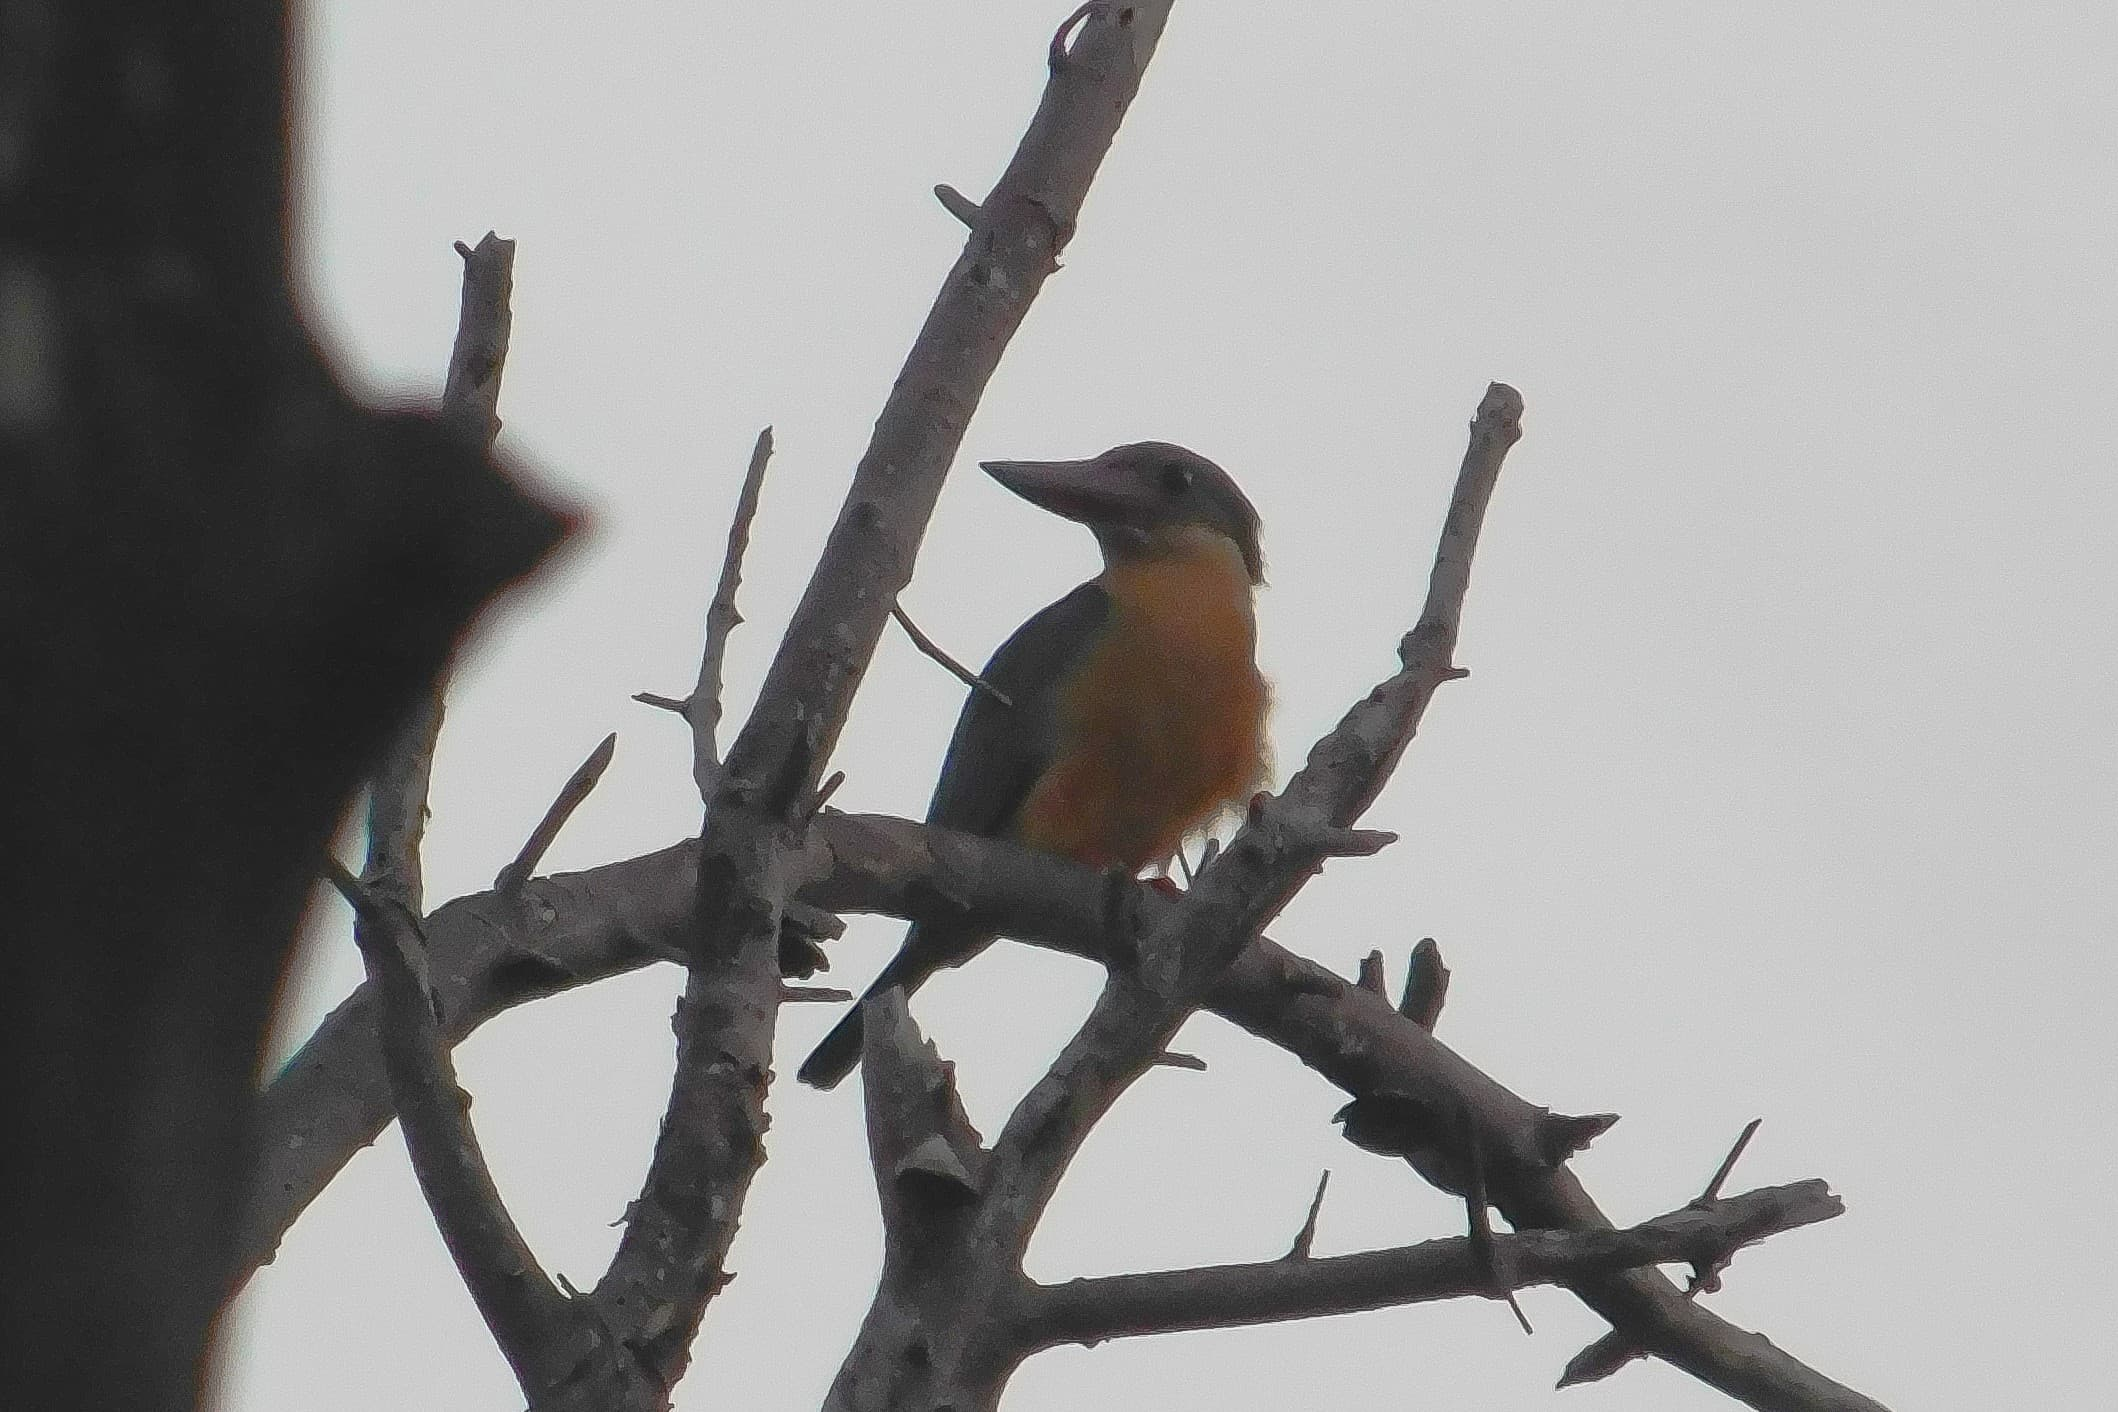
\includegraphics[width=\linewidth]{Figures/stork-billed.JPG}
    \caption[]{Stork-billed Kingfisher, Kaju kele(hotspot 2).}
    \label{fig:figure-01}
\end{figure}
